%*******10********20********30********40********50********60********70********80

% For all chapters, use the newdefined chap{} instead of chapter{}
% This will make the text at the top-left of the page be the same as the chapter

\chap{Μελλοντικές Επεκτάσεις}
%\section{Διαδραστική Επαυξημένη Πραγματικότητα}
%OTI ΔΕΝ ΕΙΠΑΜΕ ΣΤΗΝ ΕΙΣΑΓΩΓΗ ΓΙΑ AR, ΚΥΡΙΩΣ ΑΝΑΦΟΡΑ ΕΡΓΑΣΙΩΝ ΠΟΥ ΑΣΧΟΛΟΥΝΤΑΙ ΜΕ INTERACTION OF VIRTUAL OBJECTS, KAI MEΘΟΔΟΥΣ ΠΟΥ ΧΡΗΣΙΜΟΠΟΙΟΥΝΤΑΙ, ΓΙΑΤΙ ΕΙΝΑΙ ΧΡΗΣΙΜΗ Η ΑΛΛΗΛΕΠΙΔΡΑΣΗ ΣΤΟ ar


Σκοπός της παρούσας διπλωματικής εργασίας είναι η ανάπτυξη μιας εφαρμογής επαυξημένης πραγματικότητας που βασίζεται στην ανίχνευση markers, με αξιοποίηση μεθόδων αναγνώρισης χειρονομιών και όρασης υπολογιστών. Στο πλαίσιο αυτό, έγινε μία περιγραφή της έννοιας της επαυξημένης πραγματικότητας, παρουσιάστηκε το θεωρητικό υπόβαθρο των διαδικασιών οι οποίες χρησιμοποιήθηκαν για την περάτωση της εφαρμογής και έγινε αναφορά στο προγραμματιστικό μέρος, στον αισθητήρα και τα εργαλεία που χρησιμοποιήθηκαν, ενώ στο τρίτο κεφάλαιο της εργασίας παρουσιάστηκε η μεθοδολογία που ακολουθήθηκε. Παράλληλα, τα αποτελέσματα των μετρήσεων κατά την αξιολόγηση της εφαρμογής και η απάντηση των χρηστών στα ερωτηματολόγια κρίθηκαν απόλυτα ικανοποιητικά. Έχοντας ολοκληρώσει την ανάπτυξη των εφαρμογής, κρίνεται αναγκαία η επισήμανση διαφόρων προτάσεων για μελλοντική ενασχόληση και βελτίωση αυτής.


Η εφαρμογή σκακιού επαυξημένης πραγματικότητας αναγνωρίζει επιτυχώς την διάταξη των markers (markerboard) όταν αυτή τοποθετηθεί στο οπτικό πεδίο της κάμερας, ακόμη και στην περίπτωση κατά την οποία απεικονίζεται στη σκηνή ένα τμήμα της. Η σωστή αναγνώρισή των χειρονομιών "τσιμπήματος", κάτι το οποίο οφείλεται κυρίως στο χρησιμοποιούμενο αλγόριθμο ανίχνευσης και εντοπισμού του σημείου ενδιαφέροντος σε συνδυασμό με την ορθότητα των αποτελεσμάτων της βαθμονόμησης, είναι τα δύο βασικότερα στοιχεία που κρίνουν την επιτυχία επαύξησης του πραγματικού κόσμου, τη ρεαλιστικότητα της επαυξημένης σκηνής και την φυσική αλληλεπίδραση με το σύστημα. Εξάλλου, η ρεαλιστική επαύξηση της πραγματικότητας, δηλαδή η ενσωμάτωση του εικονικού μοντέλου στον τρισδιάστατο χώρο έτσι ώστε να μην ξεχωρίζει από την πραγματική σκηνή αλλά να αποτελεί μέρος της, είναι ένας από τους σημαντικότερους στόχους των εφαρμογών επαυξημένης πραγματικότητας, ο οποίος επιτεύχθηκε σε υψηλό βαθμό στην παρούσα εργασία. Παράλληλα, η αλληλεπίδραση με τα εικονικά αντικείμενα της σκηνής υλοποιήθηκε λαμβάνοντας υπόψη τις απαιτήσεις για την ανάπτυξη μιας διεπαφής με βάση την αναγνώριση χειρονομιών, ώστε οι χρήστες να αισθάνονται ότι μπορούν να χειριστούν τα πιόνια σαν να ήταν πραγματικά.


%-----


Τα εγγενή πλεονεκτήματα της μεθοδολογίας που προτείνουμε έναντι των υπόλοιπων εργασιών του επιστημονικού χώρου προκύπτουν από την απλή και γρήγορη αναγνώριση της χειρονομίας του "τσιμπήματος", όπως αναλύσαμε στο \ref{c:design}. Ταυτόχρονα, όμως, πρέπει να εξεταστεί αν με την προτεινόμενη υλοποίηση μέσω καταστάσεων αξιοποιούνται στο έπακρο οι δυνατότητες της εφαρμογής. Συνοψίζοντας, η εργασία αυτή αποτελεί μια προσπάθεια διεύρυνσης της ερευνητικής προσέγγισης του πεδίου της αναγνώρισης χειρονομιών για πειραματικώς υλοποιήσιμες εφαρμογές επαυξημένης πραγματικότητας, που βασίζονται σε βιντεοπαιχνίδια.



Με βάση τα αποτελέσματα της αξιολόγησης, οι μελλοντικές επεκτάσεις θα περιλαμβάνουν αρκετές βελτιώσεις στην πρωτότυπη έκδοση της εφαρμογής. Η βελτίωση της αναγνώρισης χειρονομιών για την αναγνώριση περισσότερων τύπων χειρονομιών και η χρήση τεχνικών machine learning για επίτευξη καλύτερων αποτελεσμάτων κρίνονται ως απαραίτητες δράσης για την περαιτέρω ανάπτυξη της εφαρμογής. Παράλληλα, καλούμαστε να βελτιώσουμε την αίσθηση του χώρου για το χρήστη, μέσω οπτικών βοηθητικών μηχανισμών με τη χρήση σκιών και φωτορεαλιστικής απεικόνισης των αντικειμένων. Υπάρχουν, μάλιστα, εργασίες που ασχολούνται με το συγκεκριμένο αντικείμενο πιο αναλυτικά \cite{Kruijff2010} \cite{Ha2014} \cite{Prachyabrued2014}.



Από την άλλη πλευρά, αρκετά πρωτότυπα εφαρμογών που έχουν υλοποιηθεί αξιοποιώντας εξελιγμένους αλγορίθμους υπολογιστικής όρασης για την απρόσκοπτη αναγνώριση χειρονομιών, ορίστηκαν ως ιδιαίτερα πολύπλοκα και με μεγάλο υπολογιστικό κόστος. Για το συγκεκριμένο λόγο, η μεθοδολογία που προτείνεται θεωρούμε ότι είναι καλύτερη, αφού δεν απαιτεί πολλούς υπολογιστικούς πόρους και είναι ιδιαίτερα απλή. Με βάση τα αποτελέσματα της αξιολόγησης, οι μελλοντικές επεκτάσεις της εφαρμογής θα μπορούσαν να περιλαμβάνουν βελτιώσεις και επιπλέον χαρακτηριστικά με στόχο την απρόσκοπτη αλληλεπίδραση σε περιβάλλοντα επαυξημένης πραγματικότητας, ώστε οι χρήστες να ζουν μια συναρπαστική εμπειρία και να "εμβυθίζονται" όσο γίνεται περισσότερο. 




%des SILTANEN
Ολόκληρος ο αλγόριθμος αναγνώρισης χειρονομίας "τσιμπήματος" έχει σχεδιαστεί και υλοποιηθεί, έτσι ώστε να είναι εύκολη η ενσωμάτωση του αισθητήρα RealSense 3D στο μπροστινό μέρος μίας συσκευής Oculus Rift. Οι αλγόριθμοι που αναπτύχθηκαν, λαμβάνουν υπόψη τους την εγωκεντρική προσέγγιση του χρήστη και την απόσταση από ένα συνηθισμένο τραπέζι και επομένως θα μπορούσαν να λειτουργήσουν χωρίς αλλαγές. Για να πραγματοποιηθεί αυτός ο συνδυασμός, στο μέλλον, πρέπει η επαυξημένη σκηνή που απεικονίζεται μέσω της OpenGL να τοποθετηθεί σε ένα texture ενός αντικειμένου Framebuffer. Έπειτα, αυτό το texture θα μπορούσε να απεικονιστεί σε μία εικονική σκηνή φτιαγμένη για το Oculus Rift και έπειτα το σύνολο της σκηνής θα μπορούσε να παραμορφωθεί με βάση το SDK του Oculus και να απεικονιστεί σε αυτό. 


Για να γίνει η εφαρμογή πιο διαδραστική και ενδιαφέρουσα, θα μπορούσαμε να χρησιμοποιήσουμε διαφορετικά τρισδιάστατα μοντέλα πιονιών σκακιού από τα κλασικά που χρησιμοποιήθηκαν. Σε μελλοντικές επεκτάσεις θα μπορούσαν να αξιοποιηθούν σύνολα πιονιών ώστε ο χρήστης να επιλέγει στην αρχή του παιχνιδιού το είδος πιονιού που του αρέσει, όπως για παράδειγμα στρατιώτες, δράκους κ.λπ.
Η χρήση πολλαπλών τρισδιάστατων μοντέλων θα μπορούσε να ενισχύσει την εμπειρία του χρήστη. Ωστόσο, θα μπορούσαμε να αξιοποιήσουμε τεχνικές animation για τη κίνηση των πιονιών και συγκεκριμένα κατά την επίθεση ενός πιονιού σε ένα άλλο και την αιχμαλώτισή του. Για παράδειγμα, αντί για εικονικά αντικείμενα τα οποία απλά εξαφανίζονται από τη σκακιέρα, θα ήταν ενδιαφέρον οι χρήστες να έβλεπαν μία έκρηξη ή μία μαγική επίθεση πάγου να εξαφανίζει το αντίπαλο πιόνι \cite{harrypotter}.


\begin{figure}[H]
    \centering
    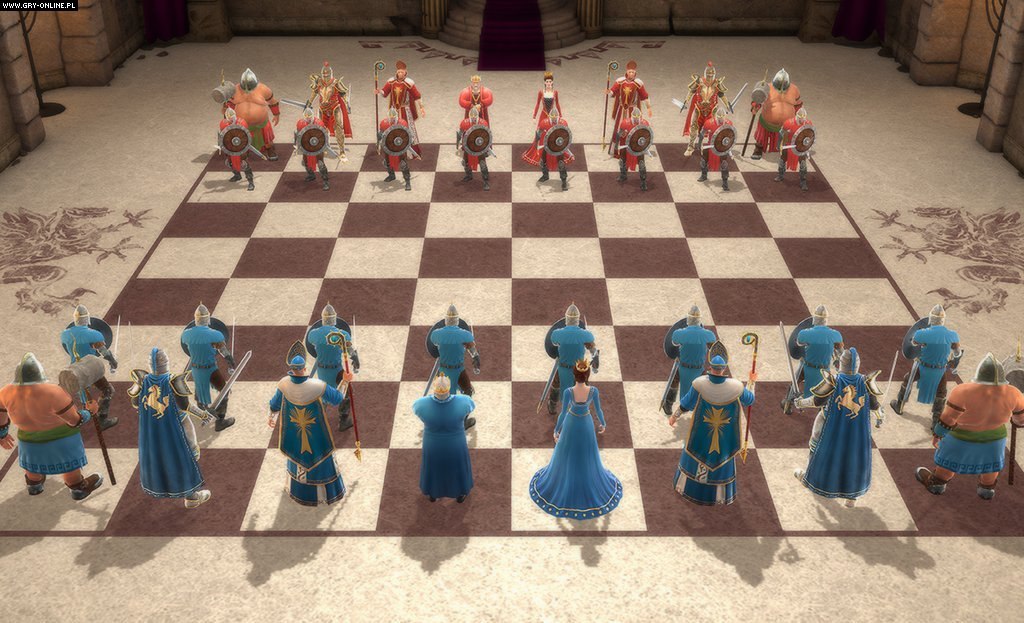
\includegraphics[width=0.55\textwidth]{Files/Figures/soldiers.jpg}
    \caption[Παράδειγμα βιντεοπαιχνιδιού που χρησιμοποιεί διαφορετικά πιόνια σκακιού]{Παράδειγμα βιντεοπαιχνιδιού που χρησιμοποιεί διαφορετικά πιόνια σκακιού}
    \label{fig:markerboard_game}
\end{figure}





Ένα πρόβλημα που καταφέραμε να αντιμετωπίσουμε, εν μέρει, έχει να κάνει με την αίσθηση βάθους του χρήστη (depth perception). Όπως αναφέρθηκε και στην προηγούμενη ενότητα, η εφαρμογή βασίστηκε στην οθόνη ενός laptop και όχι στη χρήση ενός HMD. Χρειάζεται, επομένως, ένας τρόπος ενημέρωσης του χρήστη για το σημείο στο οποίο βρίσκεται το πιόνι στον τρισδιάστατο χώρο. Για το λόγο αυτό αυτό, όταν ο χρήστης μετακινεί ένα πιόνι, εμφανίζεται με μία πράσινη ευθεία γραμμή, η κάθετη προβολή του πιονιού στη σκακιέρα. Όπως είπαν και οι χρήστες, κατά το στάδιο της αξιολόγησης, η γραμμή αυτή τους βοήθησε πολύ να καταλάβουν που βρίσκεται το πιόνι στο χώρο. Για την ενίσχυση της αίσθησης του βάθους μπορούν να χρησιμοποιηθούν κι άλλα βοηθητικά στοιχεία και να αξιοποιηθούν τεχνικές φωτορεαλιστικής απεικόνισης και εκτίμησης της θέσης πηγής φωτός της πραγματικής σκηνής \cite{frahm2005markerless} \cite{agusanto2003photorealistic} ώστε τα εικονικά αντικείμενα να σχεδιάζονται με τις σωστές σκιές.


Ένα σενάριο το οποίο θα πρέπει σίγουρα να μελετηθεί στο μέλλον, αφορά τη χρήση τεχνικών ανίχνευσης σύγκρουσης στην εφαρμογή που αναπτύχθηκε. Η αξιοποίηση τέτοιων τεχνικών μπορεί να βοηθήσει στο ρεαλισμό της εφαρμογής, αφού για παράδειγμα αν ένα πιόνι μετακινείται και συγκρουστεί με ένα άλλο στατικό πιόνι, το πιόνι θα πρέπει να πέφτει σαν να είχαμε μία πραγματική σύγκρουση με βάση τις αρχές της φυσικής. Με αυτό τον τρόπο, θα μπορούσε ο χρήστης να χρησιμοποιήσει τα χέρια του και να μετακινεί τα πιόνια, χωρίς να χρησιμοποιούνται τεχνικές αναγνώρισης της χειρονομίας του τσιμπήματος \cite{Song2008}.


Πέρα από την προσομοιώση των εικονικών αντικειμένων με χρήση των αρχών της φυσικής, έχουν προταθεί, μέσω αρκετών επιστημονικών εργασιών, προσεγγίσεις που αξιοποιούν συσκευές απτικής ανάδρασης που μπορούν να δώσουν την αίσθηση της αφής στο χρήστη όταν αγγίζει ένα εικονικό αντικείμενο. Για παράδειγμα ο Buchmann κ.α. \cite{Buchmann2004} συνέδεσαν ειδικά buzzers στα ακροδάκτυλα των χρηστών, τα οποία ουσιαστικά τους "ενημέρωναν" σχετικά με το αν άγγιξαν ένα εικονικό αντικείμενο σωστά για να το χειριστούν. Ομοίως, ένα τέτοιο σύστημα θα μπορούσε να χρησιμοποιηθεί σε συνδυασμό με την εφαρμογή που αναπτύχθηκε και παρουσιάστηκε σε αυτή τη διπλωματική εργασία.


Η πρότασή μας βρίσκεται ακόμη σε πρώιμο στάδιο και απαιτείται εντεταμένη θεωρητική εργασία για την υλοποίηση ακόμα καλύτερων αλγορίθμων που θα λειτουργούν με μεγαλύτερη ακρίβεια. Στην κατεύθυνση αυτή, πιστεύουμε ότι η ανάπτυξη συστημάτων που βασίζονται στην αναγνώριση χειρονομιών συσχετίζεται άμεσα με το μέλλον της επαυξημένης πραγματικότητας και τις διαδραστικές διεπαφές.